\section{XAML}
XML Application Markup Language\\

Ein Window besteht aus drei Dateien MainWindow.xaml, App.xaml und MainWindow.xaml.cs.
Das App.xaml ist das StartUp window welches das MainWindow.xaml aufruft. Im MainWindow.xaml wird
das ganze GUI programmiert und im MainWindow.xaml.cs ist die Schnittstelle zum Programmcode, sprich
dort werden die Funktionen aufgerufen.\\

MainWindow.xaml
\begin{lstlisting}[style=CSharp]
<Window x:Class="XAMLIntro0.MainWindow"
xmlns="http://schemas.microsoft.com/winfx/2006/xaml/presentation"
xmlns:x="http://schemas.microsoft.com/winfx/2006/xaml"
Title="XAML Demo" Height="350" Width="525">
<Button Content="Click Me"></Button>
</Window>
\end{lstlisting}

App.xaml
\begin{lstlisting}[style=CSharp]
<Application x:Class="XAMLIntro0.App"
xmlns="http://schemas.microsoft.com/winfx/2006/xaml/presentation"
xmlns:x="http://schemas.microsoft.com/winfx/2006/xaml"
StartupUri="MainWindow.xaml">
</Application>
\end{lstlisting}

MainWindow.xaml.cs
\begin{lstlisting}[style=CSharp]
using System.Windows;
namespace XAMLIntro0 {
  public partial class MainWindow : Window {
    public MainWindow()
    {
      InitializeComponent();
    }
    private void ButtonClick(object sender, RoutedEventArgs e)
    {
      System.Windows.MessageBox.Show(
      string.Format("Button Clicked {0}", e.Source));
    }
  }
}
\end{lstlisting}

\subsection{XAML Namespace \buch{p.10}}
\begin{multicols}{2}

Der XML Namespace mapt zu einem anderen CLR Namespace wie:
\begin{itemize}
  \item System.Windows
  \item System.Windows.Controls
\end{itemize}

\columnbreak

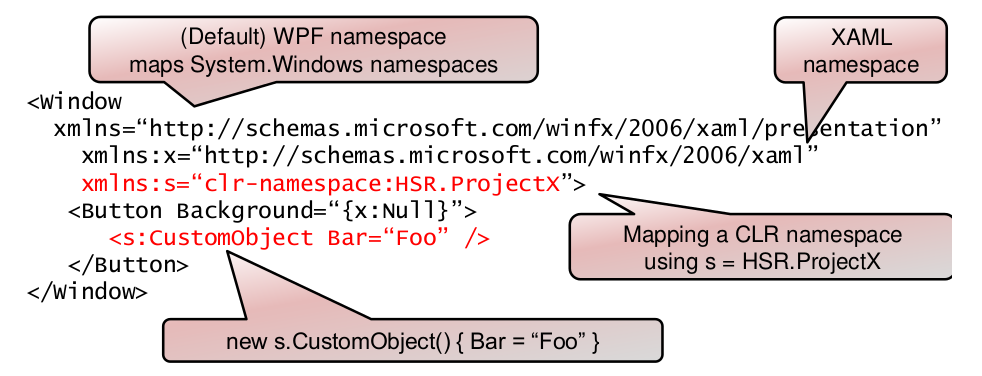
\includegraphics[width=9cm]{images/XAML/namespaces}
\end{multicols}

\subsection{WPF Controls Overview}
\begin{multicols}{4}
Display:
\begin{itemize}
  \item MediaElement
  \item Image
  \item MultiScaleImage
  \item ProgressBar
  \item Tooltip
  \item ContentControl
\end{itemize}

Control:
\begin{itemize}
  \item Button
  \item HyperlinkButton
  \item ToggleButton
  \item RepeatButton
  \item RadioButton
  \item CheckBox
  \item ComboBox
  \item TextBox
  \item TextBlock
  \item Slider
  \item DatePicker
  \item Calendar*
\end{itemize}

Items:
\begin{itemize}
  \item ListBox
  \item ItemsControl
  \item DataGrid
\end{itemize}

Layout:
\begin{itemize}
  \item Border
  \item Panel
  \item Grid
  \item Canvas
  \item StackPanel
  \item ScrollViewer
  \item TabControl
  \item GridSplitter
\end{itemize}

Popup:
\begin{itemize}
  \item Popup
  \item MessageBox
  \item FileOpenDialog
  \item PasswordBox
\end{itemize}

\end{multicols}

\subsection{Content Property}
Ein Objekt kann eingefügt werden mittels
\begin{lstlisting}[style=CSharp]
<Button Content="Button"/>
<Button>Button1</Button>
\end{lstlisting}
Wobei beides dasselbe ist.


Weitere Properties sind:\\
\begin{tabular}{lp{10cm}}
  Fill="Red" & Füllt die Fläche mit einer Farbe \\
  Width="100" & definiert die Breite (Pixel) \\
  Height="30" & definiert die Höhe (Pixel) \\
  Content="Text" & Inhalt (z.B Button Label) \\
  x:Name=''mCountValue'' IsReadOnly="True" & definiert die Variable mCountValue zum entsprechenden Objekt.
                         Diese Variable kann dann im MainWindow.xaml.cs weiterverwendet werden.\\
  Margin="5 0 0 0" & definiert den Abstand um das Objekt\\
\end{tabular}

\subsection{Funktionsaufruf mittels Button}
In MainWindow.xaml
\begin{lstlisting}[style=CSharp]
<Button Click="XXX_Click">--</Button>
\end{lstlisting}
Wobei XXX\_Click der Name der aufzurufenden Funktion ist.\\

Im File MainWindow.xaml.cs muss dann die Funktion wie folgt definiert werden
\begin{lstlisting}[style=CSharp]
private void XXX_Click(object sender, RoutedEventArgs e)
{
  mCounter.XXX();
}
\end{lstlisting}

Möchte man eine Applikation beenden kann die Funktion \textit{Close();} aufgerufen werden.

\subsection{Layouts}
\subsubsection{Layout-Canvas}
\begin{minipage}{14cm}

\begin{lstlisting}[style=CSharp]
<Window x:Class="Layouts.Canvas"
    xmlns="http://schemas.microsoft.com/winfx/2006/xaml/presentation"
    xmlns:x="http://schemas.microsoft.com/winfx/2006/xaml"
    Title="Layouts" Height="100" Width="160">
  <Grid>
    <Canvas>
      <Button Canvas.Left="10" Canvas.Top="10">
        Canvas [Left:10, Top:10]
      </Button>
      <Button Canvas.Left="10" Canvas.Top="40">
        Canvas [Left:10, Top:40]
      </Button>
    </Canvas>
  </Grid>
</Window>
\end{lstlisting}


\end{minipage}
\begin{minipage}{4cm}
  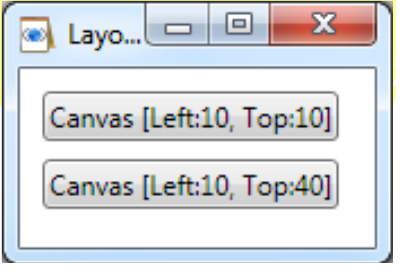
\includegraphics[width=4cm]{images/XAML/canvas}
\end{minipage}


\subsubsection{Layout-StackPanel}
\begin{minipage}{14cm}
\begin{lstlisting}[style=CSharp]
<Window x:Class="Layouts.StackPanel"
  xmlns="http://schemas.microsoft.com/winfx/2006/xaml/presentation"
  xmlns:x="http://schemas.microsoft.com/winfx/2006/xaml"
  Title="Layouts - StackPanel" Height="150" Width="250">
  <Grid>
    <StackPanel Orientation="Vertical">
      <StackPanel Orientation="Vertical">
        <Button>Button 1</Button>
        <Button>Button 2</Button>
      </StackPanel>
      <StackPanel Orientation="Horizontal">
        <Button>Button 3</Button>
        <Button>Button 4</Button>
      </StackPanel>
    </StackPanel>
  </Grid>
</Window>
\end{lstlisting}
\end{minipage}
\begin{minipage}{4cm}
  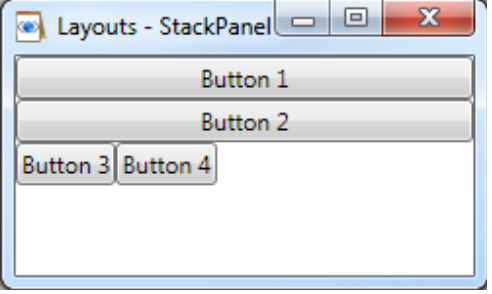
\includegraphics[width=4cm]{images/XAML/StackPanel}
\end{minipage}

\subsubsection{Layout-DockPanel}
\begin{minipage}{14cm}
\begin{lstlisting}[style=CSharp]
<Window x:Class="Layouts.DockPanel"
  xmlns="http://schemas.microsoft.com/winfx/2006/xaml/presentation"
  xmlns:x="http://schemas.microsoft.com/winfx/2006/xaml"
  Title="Layouts" Height="188" Width="300"
  >
  <Grid>
    <DockPanel>
      <Button DockPanel.Dock="Left">Button links</Button>
      <Button DockPanel.Dock="Right">Button rechts</Button>
      <Button DockPanel.Dock="Top">Button oben</Button>
      <Button DockPanel.Dock="Bottom">Button unten</Button>
    </DockPanel>
  </Grid>
</Window>
\end{lstlisting}
\end{minipage}
\begin{minipage}{4cm}
  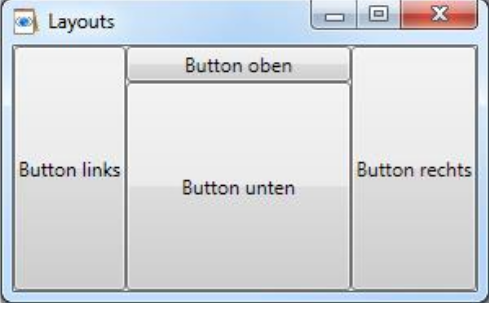
\includegraphics[width=4cm]{images/XAML/DockPanel}
\end{minipage}

\subsubsection{Layout-WrapPanel}
\begin{minipage}{14cm}
\begin{lstlisting}[style=CSharp]
<Window x:Class="Layouts.WrapPanel"
  xmlns="http://schemas.microsoft.com/winfx/2006/xaml/presentation"
  xmlns:x="http://schemas.microsoft.com/winfx/2006/xaml"
  Title="Layouts" Height="100" Width="250"
  >
  <Grid>
    <WrapPanel Orientation="Horizontal">
      <Button Width="100" Height="30">Button</Button>
      <Button Width="100" Height="30">Button</Button>
      <Button Width="100" Height="30">Button</Button>
    </WrapPanel>
  </Grid>
</Window>
\end{lstlisting}
\end{minipage}
\begin{minipage}{4cm}
  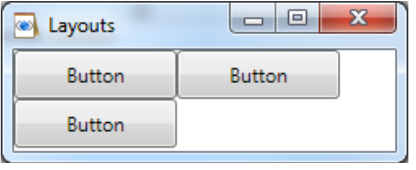
\includegraphics[width=4cm]{images/XAML/WrapPanel}
\end{minipage}

\subsubsection{Layout-TabPanel}
\begin{minipage}{14cm}
\begin{lstlisting}[style=CSharp]
<Window x:Class="Layouts.TabPanel"
  xmlns="http://schemas.microsoft.com/winfx/2006/xaml/presentation"
  xmlns:x="http://schemas.microsoft.com/winfx/2006/xaml"
  Title="Layouts - TabPanel" Height="100" Width="300">
  <Grid>
    <TabPanel>
      <TabControl>
        <TabItem Header="Header 1">
          <Button>Button 1</Button>
        </TabItem>
        <TabItem Header="Header 2">
          <Button>Button 2</Button>
        </TabItem>
      </TabControl>
    </TabPanel>
  </Grid>
</Window>
\end{lstlisting}
\end{minipage}
\begin{minipage}{4cm}
  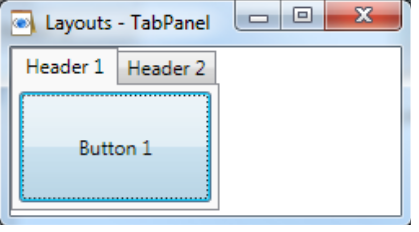
\includegraphics[width=4cm]{images/XAML/TabPanel}
\end{minipage}

\subsubsection{Layout-Viewbox}
\begin{minipage}{14cm}
\begin{lstlisting}[style=CSharp]
<Window x:Class="Layouts.ViewBox"
  xmlns="http://schemas.microsoft.com/winfx/2006/xaml/presentation"
  xmlns:x="http://schemas.microsoft.com/winfx/2006/xaml"
  Title="Layouts - Viewbox" Height="100" Width="500">
  <Grid>
    <Viewbox>
      <TextBlock>
        Franz jagt im komplett verwahrlosten Taxi quer durch Bayern.
        Franz jagt im komplett verwahrlosten Taxi quer durch Bayern.
      </TextBlock>
    </Viewbox>
  </Grid>
</Window>
\end{lstlisting}
\end{minipage}
\begin{minipage}{4cm}
  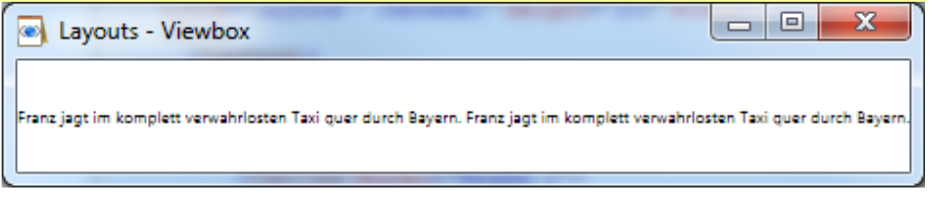
\includegraphics[width=4cm]{images/XAML/Viewbox}
\end{minipage}

\subsubsection{Layout-Grid}
\begin{minipage}{14cm}
\begin{lstlisting}[style=CSharp]
<Window x:Class="Layouts.Grid"
  xmlns="http://schemas.microsoft.com/winfx/2006/xaml/presentation"
  xmlns:x="http://schemas.microsoft.com/winfx/2006/xaml"
  Title="Layouts - Grid" Height="300" Width="300">
  <Grid><Grid.RowDefinitions>
    <RowDefinition Height="20" />
    <RowDefinition Height="0.5*" />
    <RowDefinition Height="0.4*" />
    <RowDefinition Height="0.1*" />
  </Grid.RowDefinitions><Grid.ColumnDefinitions>
    <ColumnDefinition Width="0.5*" />
    <ColumnDefinition Width="0.5*" />
  </Grid.ColumnDefinitions>
    <Button Name="btnButton1" Grid.Row="0"
    Grid.Column="1">Button 1</Button>
    <Button Name="btnButton2" Grid.Row="1"
    Grid.Column="0" Grid.ColumnSpan="2">
    Button 2</Button>
    <Button Name="btnButton3" Grid.Row="2"
    Grid.Column="0" Grid.RowSpan="2">
    Button3 </Button>
  </Grid>
</Window>
\end{lstlisting}
\end{minipage}
\begin{minipage}{4cm}
  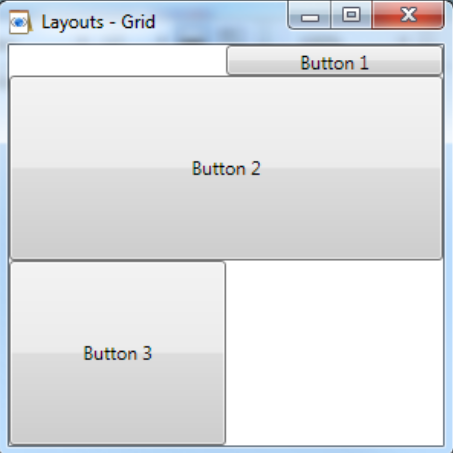
\includegraphics[width=4cm]{images/XAML/Grid}
\end{minipage}


